% !TEX TS-program = xelatex
\documentclass[aspectratio=169]{beamer}

% --- THEME & LAYOUT ---
\usetheme[numbering=fraction,progressbar=head]{metropolis}
\setbeamersize{text margin left=8mm,text margin right=8mm}

% --- CUSTOM FOOTER WITH TLP MARKING ---
\setbeamertemplate{frame footer}{\textbf{TLP:CLEAR} -- Information may be shared freely without restriction.}
\setbeamercolor{frame footer}{fg=cyber-accent}

\usepackage{amsmath}

% --- FONTS (XeLaTeX) ---
\usepackage{fontspec}
\setsansfont[
  Ligatures=TeX, Scale=1.02,
  BoldFont = {IBM Plex Sans Bold},
  ItalicFont = {IBM Plex Sans Italic}
]{IBM Plex Sans}
\setmonofont{IBM Plex Mono}

% --- ICONS ---
\usepackage{fontawesome5}

% --- COLORS (cyber palette) ---
\definecolor{cyber-bg}{HTML}{0B0F14}
\definecolor{cyber-ink}{HTML}{E6EEF5}
\definecolor{cyber-accent}{HTML}{217EAA}
\definecolor{cyber-mid}{HTML}{7D9CB7}
\definecolor{cyber-soft}{HTML}{8CA4AC}
\setbeamercolor{normal text}{fg=cyber-ink,bg=cyber-bg}
\setbeamercolor{frametitle}{fg=cyber-ink,bg=cyber-bg}
\setbeamercolor{progress bar}{fg=cyber-accent,bg=cyber-soft}
\setbeamercolor{alerted text}{fg=cyber-accent}

% --- LINKS ---
\hypersetup{colorlinks=true, linkcolor=cyber-accent, urlcolor=cyber-accent}

% --- CODE / BOXES ---
\usepackage{listings}
\lstset{
  basicstyle=\ttfamily\footnotesize,
  backgroundcolor=\color{black!5},
  frame=single, rulecolor=\color{cyber-soft},
  keywordstyle=\color{cyber-accent}\bfseries,
  commentstyle=\color{cyber-soft},
  showstringspaces=false
}
\usepackage[most]{tcolorbox}
\usepackage{qrcode}
\usetikzlibrary{fit,arrows.meta,positioning}
\tcbset{colback=black!5!cyber-bg, colframe=cyber-soft, coltext=cyber-ink, boxsep=1mm, left=2mm, right=2mm}

% --- PDF TOOLS ---

% --- GRAPHICS ---
\usepackage{graphicx}

% --- SPEAKER NOTES ---
\usepackage{pgfpages}
% \setbeameroption{hide notes}
% \setbeameroption{show notes}
% \setbeameroption{show only notes}

% --- SPACING IMPROVEMENTS ---
\setbeamertemplate{itemize/enumerate body begin}{\vspace{-0.5ex}}
\setbeamertemplate{itemize/enumerate subbody begin}{\vspace{-0.5ex}}

% --- TITLE INFO ---
\title{\texorpdfstring{\raisebox{-1.65em}{\includegraphics[trim=9 59 4 43, clip, height=4em]{../../../images/logos/range42.png}}\;}{Range42 -- }Project Overview}
\subtitle{Open-Source Cyber Range Platform for Collaborative Security Training}
\author{\texorpdfstring{}{Range42 Team: }%
  \texorpdfstring{\raisebox{-0.75em}{\includegraphics[trim=109 152 109 186, clip, height=1.9em]{../../../images/logos/nc3.png}}\;}{}NC3.LU
  \quad+\quad
  \texorpdfstring{\raisebox{-0.75em}{\includegraphics[trim=92 108 92 58, clip, height=2.2em]{../../../images/logos/digisquad.pdf}}\;}{}DIGISQUAD
  \texorpdfstring{\\[0.4em]\makebox[1.6em][l]{\faGithub}\href{https://github.com/range42}{github.com/range42}%
    \\[0.2em]\makebox[1.6em][l]{\faGlobe}\href{https://range42.lu/}{range42.lu}}{}}
\date{\vspace*{2.5em}November 2026}

% Notes pages: Beamer's default note template, but the header shows the frame title.
% The default uses \insertshortframetitle, which is empty on notes pages here.
% The thumbnail is the real page of the slides PDF (built first by make): Beamer's own
% thumbnail drops the footer and shows uncoloured text in the dark note colour.
% ponytail: page = frame number + 1 holds while the title is the only unnumbered frame and
% no frame has overlays; with overlays or appendix frames, map pages through labels instead.
\makeatletter
\setbeamertemplate{note page}{%
  {%
    \scriptsize
    \usebeamerfont{note title}\usebeamercolor[fg]{note title}%
    \ifbeamercolorempty[bg]{note title}{}{%
      \insertvrule{.25\paperheight}{note title.bg}%
      \vskip-.25\paperheight%
      \nointerlineskip%
    }%
    \vbox{
      \hfill\IfFileExists{range42-overview-2026-11.pdf}{\includegraphics[width=0.25\paperwidth,page=\numexpr\insertframenumber+1\relax]{range42-overview-2026-11.pdf}}{\insertslideintonotes{0.25}}\hskip-\Gm@rmargin\hskip0pt%
      \vskip-0.25\paperheight%
      \nointerlineskip
      \begin{pgfpicture}{0cm}{0cm}{0cm}{0cm}
        \begin{pgflowlevelscope}{\pgftransformrotate{90}}
          {\pgftransformshift{\pgfpoint{-2cm}{0.2cm}}%
          \pgftext[base,left]{\usebeamerfont{note date}\usebeamercolor[fg]{note date}\the\year-\ifnum\month<10\relax0\fi\the\month-\ifnum\day<10\relax0\fi\the\day}}
        \end{pgflowlevelscope}
      \end{pgfpicture}}
    \nointerlineskip
    \vbox to .25\paperheight{\vskip0.5em
      \hbox{\insertshorttitle[width=0.75\textwidth]}%
      \setbox\beamer@tempbox=\hbox{\insertframetitle}%
      \hbox{\ifdim\wd\beamer@tempbox>1pt{\hskip4pt\raise3pt\hbox{\vrule
            width0.4pt height7pt\vrule width 9pt
            height0.4pt}}\hskip1pt\hbox{\normalsize\bfseries\insertframetitle}\fi%
      }%
      \vfil}%
  }%
  \ifbeamercolorempty[bg]{note page}{}{%
    \nointerlineskip%
    \insertvrule{.75\paperheight}{note page.bg}%
    \vskip-.75\paperheight%
  }%
  \vskip.25em
  \nointerlineskip
  {\footnotesize\insertnote\par}
}
\makeatother

\begin{document}

% === TITLE ===
\begin{frame}[plain,noframenumbering]
  \titlepage
  \note[item]{Goal: 20-minute overview of the Range42 project as of November 2026: what it is, why it exists, how it is built, where it goes.}
  \note[item]{Audience: cybersecurity professionals, government, partners.}
\end{frame}

% === WHAT IS RANGE42 ===
% #1 = icon, #2 = statement, on one line.
\newcommand{\whatitem}[2]{{\Large #1\;\;\textbf{#2}}}

\begin{frame}{What is Range42?}
  \whatitem{\faCrosshairs}{Cyber Training \& Exercise Platform}
  \par\bigskip
  \begin{itemize}
    \item \makebox[1.6em][l]{\faIcon{shield-alt}}Blue-team / red-team exercises
    \item \makebox[1.6em][l]{\faFlag}Capture The Flag (CTF) challenges
    \item \makebox[1.6em][l]{\faChessKnight}Tabletop cyber exercises (TTX)
    \item \makebox[1.6em][l]{\faExclamationTriangle}Real-world incident simulation
  \end{itemize}
  \note[item]{Key message: Range42 is one platform for every kind of cyber exercise, from hands-on labs to tabletop.}
  \note[item]{Blue / red team: trainee environments for attack and defence; admin services such as Wazuh (detection) and MISP (threat intelligence).}
  \note[item]{CTF: catalog challenges (CVE, malware, misconfiguration) with themed web front-ends, e.g.\ a fake hospital or a fake bank.}
  \note[item]{TTX: tabletop exercises with injects and group responses, run with table42 (presented later).}
  \note[item]{Real-world incidents simulated safely: isolated labs, snapshots to reset, and telemetry to observe what happens.}
\end{frame}

% === WHY RANGE42 ===
\begin{frame}{Why Range42?}
  \centering
  \renewcommand{\arraystretch}{1.9}
  \begin{tabular}{@{}l@{\;\;}l@{\quad}c@{\quad}l@{}}
    & {\color{cyber-soft}\small\bfseries TODAY'S CYBER RANGES} & & {\small\bfseries RANGE42} \\
    \faLock          & Closed, proprietary software        & \faArrowRight & \textbf{Open source} \\
    \faCoins         & High licence and platform costs     & \faArrowRight & \textbf{No licence fees} \\
    \faLink          & Dependence on external providers & \faArrowRight & \textbf{Digital sovereignty} \\
    \faTools         & Scenarios locked inside the platform & \faArrowRight & \textbf{Portable labs, as code} \\
  \end{tabular}
  \note[item]{Key message: realistic cyber training should not depend on a closed vendor.}
  \note[item]{Main commercial ranges, in Europe (Airbus CyberRange, CDeX, CybExer) and in the US (SimSpace, Cyberbit), are proprietary: you cannot read, change or extend them. Range42 is open source (GPL-3.0).}
  \note[item]{Costs: commercial ranges are sold as licences or subscriptions (SaaS access stops when the subscription ends). Range42 has no licence fees: it runs on your own Proxmox VE hardware.}
  \note[item]{Digital sovereignty: even on-premise, commercial ranges depend on the vendor for licences, updates and new scenarios (e.g.\ Airbus sells scenario development as consulting). With Range42, infrastructure, code and data stay under your control.}
  \note[item]{Scenarios: competitors have scenario builders, but scenarios stay inside their platform. Range42 labs are code, versioned in Git and rebuilt identically from any commit.}
\end{frame}

\begin{frame}{How does Range42 work?}
  \noindent{\large\faPuzzlePiece\;\textbf{Modular Cyber Range}}
  \par\medskip
  \centering
  \begin{tikzpicture}[
      font=\footnotesize,
      blk/.style={draw=cyber-accent, fill=cyber-accent!25!cyber-bg, text=cyber-ink,
                  rounded corners=2pt, align=center, minimum height=0.7cm, inner sep=2pt},
      part/.style={blk, draw=cyber-mid, fill=cyber-mid!25!cyber-bg, font=\scriptsize},
      lane/.style={text=cyber-soft, font=\tiny\bfseries, anchor=east},
      ztitle/.style={text=cyber-ink, font=\scriptsize\bfseries},
      zbox/.style={draw=cyber-soft, dashed, rounded corners=3pt, inner sep=4pt},
      zoom/.style={cyber-soft, dashed},
    ]
    % The range: a stack of blocks
    \node[blk, minimum width=2.5cm] (ui)  at (1.3,3.3) {\faProjectDiagram\; Deployer UI};
    \node[blk, minimum width=2.5cm] (cli) at (3.9,3.3) {\faTerminal\; Deployer CLI};
    \node[blk, minimum width=5.1cm] (api) at (2.6,2.3) {\faPlug\; API};
    \node[blk, minimum width=5.1cm] (aut) at (2.6,1.3) {\raisebox{-0.2em}{\includegraphics[height=1.1em]{../../../images/logos/ansible.pdf}}\; Playbooks};
    \node[blk, minimum width=5.1cm] (pve) at (2.6,0.3)
      {\raisebox{-0.2em}{\includegraphics[height=1.1em]{../../../images/logos/proxmox.pdf}}\; Virtual Environment};
    \node[lane] at (0,3.3) {INTERFACES};
    \node[lane] at (0,2.3) {CORE};
    \node[lane] at (0,1.3) {AUTOMATION};
    \node[lane] at (0,0.3) {INFRASTRUCTURE};

    % Zoom 1: the API is made of services
    \node[part, minimum width=2.9cm, minimum height=0.55cm] (a1) at (8.1,3.6)  {\faLock\; Gateway};
    \node[part, minimum width=2.9cm, minimum height=0.55cm] (a2) at (11.25,3.6) {\faIcon{exchange-alt}\; REST API};
    \node[part, minimum width=2.9cm, minimum height=0.55cm] (a3) at (8.1,2.95)  {\faPlay\; Job runner};
    \node[part, minimum width=2.9cm, minimum height=0.55cm] (a4) at (11.25,2.95) {\faBroadcastTower\; Live status};
    \node[zbox, fit=(a1)(a2)(a3)(a4)] (apiz) {};
    \node[ztitle, above=0pt of apiz.north] {API = services};

    % Zoom 2: a scenario is made of bundles
    \node[part, minimum width=2.9cm, minimum height=0.55cm] (b1) at (8.1,1.45)  {\faServer\; VM / Container};
    \node[part, minimum width=2.9cm, minimum height=0.55cm] (b2) at (11.25,1.45) {\faIcon{shield-alt}\; Firewall};
    \node[part, minimum width=2.9cm, minimum height=0.55cm] (b3) at (8.1,0.8)   {\faEye\; Admin service};
    \node[part, minimum width=2.9cm, minimum height=0.55cm] (b4) at (11.25,0.8)  {\faFlag\; CTF challenge};
    \node[zbox, fit=(b1)(b2)(b3)(b4)] (scn) {};
    \node[ztitle, above=0pt of scn.north] {Scenario = bundles};
    \node[below=1pt of scn.south, text=cyber-soft, font=\tiny]
      {\faRecycle\; reusable bundles, built from the catalog};

    \draw[zoom] (api.north east) -- (apiz.north west);
    \draw[zoom] (api.south east) -- (apiz.south west);
    \draw[zoom] (aut.north east) -- (scn.north west);
    \draw[zoom] (aut.south east) -- (scn.south west);
  \end{tikzpicture}
  \note[item]{Key message: Range42 is a set of blocks. Each block has one role and evolves on its own.}
  \note[item]{Interfaces: Deployer UI (visual lab design) and Deployer CLI (\texttt{range42-context}, daily operations). One deployer, several Proxmox clusters.}
  \note[item]{API: gateway (authentication, access control lists (ACL)), REST API (OpenAPI), job runner (ansible-runner), live status (WebSocket).}
  \note[item]{Playbooks: Ansible does the work; secrets in Ansible Vault. A scenario is a set of bundles: VM/container, firewall, admin service, CTF challenge.}
  \note[item]{Bundles are reusable (e.g.\ Wazuh), built from the catalog: Ansible roles, Docker Compose stacks, gamification.}
  \note[item]{Proxmox VE hosts the VMs, LXC (Linux Containers) containers and SDN (software-defined networking) networks, created via its API.}
  \note[item]{Everything is code, versioned in Git: any lab is rebuilt identically from any commit; changes are reviewed.}
\end{frame}

% === WHAT CAN YOU RUN ===
% #1 = icon, #2 = category, #3 = examples.
\newcommand{\runitem}[3]{\makebox[1.8em][l]{\Large #1}\parbox[t]{\dimexpr\linewidth-1.8em}{\raggedright{\large\textbf{#2}}\par\smallskip{\small #3\strut}}}

\begin{frame}{What can you run?}
  \vspace*{1em}
  \begin{tabular}{@{}p{0.47\textwidth}@{\hspace{0.06\textwidth}}p{0.47\textwidth}@{}}
    \runitem{\faServer}{Infrastructure}{Custom networks, Linux hosts, Windows AD} &
    \runitem{\faComments}{Product labs}{Real-world tools, e.g.\ Nextcloud, Gitea, Mattermost} \\
    \noalign{\vspace{2.5em}}
    \runitem{\faEye}{Detection \& defence}{SIEM and endpoint monitoring, e.g.\ Wazuh} &
    \runitem{\faBug}{Offensive \& CTF}{Vulnerable and misconfigured services, themed web fronts} \\
  \end{tabular}
  \note[item]{Key message: ready-to-deploy labs, all built from the reusable bundles of the previous slide.}
  \note[item]{Infrastructure: any number of SDN subnets, isolated on demand (NAT (network address translation) toggle, Proxmox firewall). Linux hosts (Debian, Ubuntu, Alpine). Windows Active Directory (AD): domain controller and client.}
  \note[item]{Product labs: any tool packaged as a bundle (Docker Compose or VM), for admin training or as targets. Today: MISP, Gitea, Mattermost, Nextcloud, Rocket.Chat.}
  \note[item]{Detection: any SIEM (security information and event management) or monitoring tool packaged as a bundle. Today: Wazuh server and agents.}
  \note[item]{CTF: vulnerable services (known CVEs) and misconfigured services, each a reusable bundle. Themed web fronts (e.g.\ a fake hospital or bank) make the challenge realistic.}
\end{frame}

% === SEE IT ===
\begin{frame}{See it: Deployer UI}
  \begin{columns}[c]
    \column{0.69\textwidth}
    \centering
    \includegraphics[width=\linewidth,height=0.80\textheight,keepaspectratio]{../../../images/screenshots/deployer-ui-design.png}
    \column{0.28\textwidth}
    \raggedright
    {\large\textbf{\faDrawPolygon\; Design the lab}}\par\bigskip
    {\large\textbf{\faPlay\; Deploy and follow it live}}
  \end{columns}
  \note[item]{Key message: no YAML needed to build a lab. The UI and the CLI run the same playbooks on the same Proxmox.}
  \note[item]{Design: drag VMs, containers and networks on a canvas, attach catalog bundles, save the lab as a Git revision.}
  \note[item]{Deploy: preflight checks before any change, then live progress, logs and events.}
\end{frame}

% === AROUND THE RANGE ===
\begin{frame}{Around the Range}
  \runitem{\faChessKnight}{table42}{Run tabletop exercises (TTX) digitally, every decision kept for the debrief}
  \par\vspace{2.2em}
  \runitem{\faIcon{file-alt}}{Reporting tool}{Evaluate teams on their analysis, not only on flags}
  \par\vspace{2.2em}
  {\small\color{cyber-soft}\faPlug\; Both also work with any cyber range.}
  \note[item]{Key message: the range is the infrastructure; these tools cover the exercise itself.}
  \note[item]{table42: a TTX on slides and paper loses decisions. Here the facilitator pushes injects, each group answers in the app, and everything is exported for the debrief.}
  \note[item]{Reporting tool: real incidents end with a report. Teams write theirs during the exercise; organisers review, validate and evaluate them in one place, with the same criteria for every team.}
  \note[item]{Both tools can be used with any cyber range, or without one.}
\end{frame}

% === TIMELINE ===
% x = position on the axis (ordered, not to scale). #1 = position, #2 = date, #3 = text.
\newcommand{\tlup}[3]{\draw[cyber-soft] (#1,0) -- (#1,0.7) node[tlev, above] {{\bfseries\color{cyber-accent}#2}\\#3}; \node[tldot] at (#1,0) {};}
\newcommand{\tldown}[3]{\draw[cyber-soft] (#1,0) -- (#1,-0.7) node[tlev, below] {{\bfseries\color{cyber-accent}#2}\\#3}; \node[tldot] at (#1,0) {};}

\begin{frame}{Timeline}
  \centering
  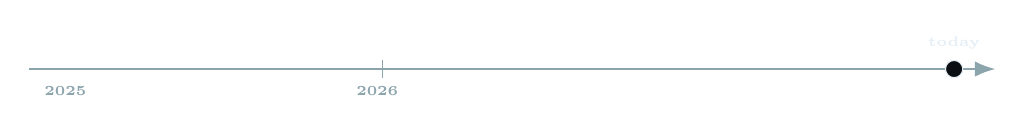
\begin{tikzpicture}[x=0.66cm, y=1.1cm,
      tlev/.style={align=center, text width=2.8cm, font=\scriptsize, text=cyber-ink, inner sep=1pt, execute at begin node={\hyphenpenalty 10000\exhyphenpenalty 10000}},
      tldot/.style={circle, fill=cyber-accent, inner sep=2.2pt},
    ]
    \draw[cyber-soft, line width=1pt, -{Latex}] (-0.8,0) -- (17.8,0);
    \foreach \m/\y in {0/2025, 6/2026}
      \node[font=\tiny\bfseries, text=cyber-soft] at (\m-0.1,-0.25) {\y};
    \draw[cyber-soft] (6,-0.1) -- (6,0.1);

    \tlup{0}{May 2025}{Project start}
    \tldown{3.5}{Jul -- Sep 2025}{Core platform: interface, API, automation}
    \tlup{7.5}{Mar 2026}{Guided installation}
    \tldown{10.5}{Apr -- Jun 2026}{Public website and documentation}
    \tlup{13.5}{Aug -- Sep 2026}{Configurable networks and firewall}
    \tldown{15.5}{Oct 2026}{Exercise tooling}

    \node[circle, draw=cyber-ink, fill=cyber-bg, inner sep=2.2pt] at (17,0) {};
    \node[font=\tiny\bfseries, text=cyber-ink] at (17,0.3) {today};
  \end{tikzpicture}
  \note[item]{Key message: 18 months from the first commit to a usable cyber range.}
  \note[item]{May 2025: GitHub organisation (23 May), first repositories: catalog, playbooks, Proxmox controller role.}
  \note[item]{Jul -- Sep 2025: Deployer UI (29 Jul), first CTF Docker stacks (4 Aug), backend API (3 Sep), API gateway (22 Sep).}
  \note[item]{Mar 2026: setup wizard and \texttt{range42-context} CLI (30 Mar).}
  \note[item]{Apr -- Jun 2026: website (17 Apr), documentation site (28 Jun).}
  \note[item]{Aug -- Sep 2026: Proxmox SDN networks (18 Aug) and firewall (4 Sep) in every deployment.}
  \note[item]{Oct 2026: exercise tooling: reporting tool (started 9 Jun), table42 (10 Oct).}
\end{frame}

% === TODAY VS TOMORROW ===
\begin{frame}{Today vs.\ Tomorrow}
  \begin{columns}[T]
    \column{0.48\textwidth}
    {\large\textbf{\faCheckCircle\; Today}}
    \begin{itemize}
      \item Guided install and operations
      \item Visual lab designer
      \item Configurable networks and firewall
      \item Ready-to-deploy labs
      \item TTX and reporting tools
    \end{itemize}
    \column{0.48\textwidth}
    {\large\textbf{\faRocket\; Tomorrow}}
    \begin{itemize}
      \item Trainee workstations
      \item Red / blue exercises with scoring
      \item Forensics and IR labs
      \item ICS and IoT scenarios
      \item Catalog sharing
    \end{itemize}
  \end{columns}
  \note[item]{Key message: the foundation works today; the next steps add exercise content and scale.}
  \note[item]{Today: everything shown in this talk. Install and operate, design labs visually (saved as code), configure networks and firewall, deploy infrastructure, product, detection and CTF labs, run TTX and reporting.}
  \note[item]{Tomorrow: trainee workstations for hands-on exercises, red / blue exercises with a scoreboard, forensics and incident-response (IR) labs, scenarios for industrial control systems (ICS), their supervision (SCADA) and IoT, a federated catalog to share bundles between organisations.}
\end{frame}

% === ROADMAP ===
\begin{frame}{Roadmap}
  \begin{tabular}{@{}p{0.53\textwidth}@{\hspace{0.03\textwidth}}p{0.44\textwidth}@{}}
    \runitem{\faIcon{shield-alt}}{Core Stabilisation \& Hardening}{Lock the architecture, validate deployments} &
    \runitem{\faSync}{State Management (DLSE)}{Labs always match their code} \\
    \noalign{\vspace{1.3em}}
    \runitem{\faDesktop}{End-User Interfaces}{Visualise, modify, control live labs} &
    \runitem{\faUserGraduate}{Student-Facing Services}{Grow the catalog, services built into labs} \\
    \noalign{\vspace{1.3em}}
    \runitem{\faIndustry}{Industrial \& IoT}{OT / ICS labs with real hardware} &
    \runitem{\faUsers}{Open-Source Ecosystem}{MISP, Kunai and more as managed labs} \\
  \end{tabular}
  \note[item]{Key message: six development axes guide the next steps of the project.}
  \note[item]{Core Stabilisation \& Hardening: lock the architecture and the installation, validate cold deployments, align CLI, UI and API.}
  \note[item]{State Management (DLSE): Desired / Live State Engine. It compares running labs with the target state, corrects the drift, keeps an audit trail.}
  \note[item]{End-User Interfaces: for instructors and students, not only operators. Visualise the deployed state, then modify and redeploy, then limited live control.}
  \note[item]{Student-Facing Services: Git, chat and file sharing exist today as standalone labs. Next: grow the catalog and run these services inside exercise labs, per class or per lab.}
  \note[item]{Industrial \& IoT: from IT to operational technology (OT / ICS) with real industrial components. Prototype first, then a go / no-go decision.}
  \note[item]{Open-Source Ecosystem: existing open-source tools (MISP, Kunai) as managed, reproducible labs. Later: synergy with NGSOTI (Next Generation Security Operator Training Infrastructure), federated catalogs.}
\end{frame}

% === GET INVOLVED ===
\begin{frame}{Get Involved}
  \vspace*{0.9em}
  \begin{columns}[c]
    \column{0.62\textwidth}
    \runitem{\faBoxOpen}{Content}{Scenarios, bundles, CTF challenges}
    \par\vspace{0.9em}
    \runitem{\faCode}{Code}{Automation, API, interfaces}
    \par\vspace{0.9em}
    \runitem{\faBook}{Documentation and testing}{Guides, bug reports, feedback}
    \par\vspace{0.9em}
    \runitem{\faHandshake}{Partnerships}{Use it, share your needs}
    \column{0.36\textwidth}
    \centering
    \colorbox{white}{\qrcode[height=2.6cm]{https://github.com/range42}}
    \par\medskip
    {\small
    \begin{tabular}{@{}c@{\;\;}l@{}}
      \faGithub   & \href{https://github.com/range42}{github.com/range42} \\
      \faGlobe    & \href{https://range42.lu/}{range42.lu} \\
      \faBook     & \href{https://docs.range42.lu/}{docs.range42.lu} \\
      \faEnvelope & \href{mailto:range42@nc3.lu}{range42@nc3.lu} \\
    \end{tabular}}
  \end{columns}
  \note[item]{Key message: Range42 is open source; every contribution moves the platform forward.}
  \note[item]{Content: new scenarios, bundles for new services and apps, CTF challenges.}
  \note[item]{Code: Ansible roles and automation, backend API, Deployer UI and CLI.}
  \note[item]{Documentation and testing: guides on docs.range42.lu, bug reports and feedback on GitHub.}
  \note[item]{Partnerships: organisations can deploy Range42 for their own training and tell us what they need.}
  \note[item]{The QR code opens github.com/range42. Contact: range42@nc3.lu.}
\end{frame}

% === CLOSING ===
\begin{frame}{}
  \centering
  \includegraphics[trim=9 59 4 43, clip, height=5em]{../../../images/logos/range42.png}
  \par\bigskip
  {\Huge\bfseries Thank you}
  \par\medskip
  {\Large Questions?}
  \par\vspace{1.5em}
  {\small
  \faGithub\; \href{https://github.com/range42}{github.com/range42}\qquad
  \faGlobe\; \href{https://range42.lu/}{range42.lu}\qquad
  \faEnvelope\; \href{mailto:range42@nc3.lu}{range42@nc3.lu}}
  \note[item]{Thank the audience and open the questions.}
  \note[item]{Likely questions: Windows AD status, which repositories are public, comparison with commercial ranges, how to try it (docs.range42.lu).}
\end{frame}

\end{document}
